\documentclass[a4paper,10pt]{report}
% Dino Anastasopoulos, 2021

% Include Packages
%\usepackage[a4paper,inner=3.5cm,outer=2.5cm,top=2.5cm,bottom=2.5cm]{geometry}  % Set page margins
\usepackage{fullpage}
\usepackage{float}                  % Allows 'Here and Only Here' [H] for Floats
\usepackage[hyphens]{url}           % \url{} command
\usepackage{charter}                  % Set font to Times
\usepackage{graphicx}               % \includegraphics
%\usepackage{subfigure}              % Allow subfigures
\usepackage{caption}
\usepackage{subcaption}
\usepackage{enumerate}


\setlength{\columnsep}{1.5cm}


\usepackage{amsmath}
\usepackage{amssymb}
\usepackage{amsthm}
\usepackage{booktabs}
\usepackage{parskip}
\usepackage[all]{nowidow}
\setnoclub[2]
\setnowidow[2]

% Referencing
% Provides \Vref and \vref to indicate where a reference is.
\usepackage{varioref} 
% Hyperlinks references
\usepackage[bookmarks=true,bookmarksopen=true]{hyperref} 
% Provides \Cref, \cref, \Vref, \vref to include the type of reference: fig/eqn/tbl
\usepackage{cleveref} 
\usepackage{pgfgantt}

% Setup Hyperref
\hypersetup{
	colorlinks   = true,              %Colours links instead of ugly boxes
	urlcolor     = blue,              %Colour for external hyperlinks
	linkcolor    = blue,              %Colour of internal links
	citecolor    = blue                %Colour of citations
}
% Names for Clever Ref
\crefname{table}{table}{tables}
\Crefname{table}{Table}{Tables}
\crefname{figure}{figure}{figures}
\Crefname{figure}{Figure}{Figures}
\crefname{equation}{equation}{equations}
\Crefname{equation}{Equation}{Equations}

% Wits Citation Style
\usepackage{natbib} \input{natbib-add}
\bibliographystyle{named-wits}
\bibpunct{[}{]}{;}{a}{}{}  % to get correct punctuation for bibliography
\setlength{\skip\footins}{1.5cm}
\newcommand{\citets}[1]{\citeauthor{#1}'s \citeyearpar{#1}}
\renewcommand\bibname{References}  

\pagestyle{headings}

\pagestyle{plain}
\pagenumbering{roman}

\newenvironment{declaration}{\ \vfill\begin{center}\textbf{Declaration}\end{center}\addcontentsline{toc}{section}{Declaration}}{\vfill\vfill\newpage}

\begin{document}
	\onecolumn
	\thispagestyle{empty}
	
	\setcounter{page}{0}
	\addcontentsline{toc}{chapter}{Preface}
	
	\begin{center}
		\vfill
		{
			\huge \bf \textsc{Cartoonify: \\Artistic Effects Using Image Processing Techniques}\\
			\large School of Computer Science \& Applied Mathematics\\
			\large University of the Witwatersrand\\[20pt]
			\normalsize
			Dino Anastasopoulos\\
			\today
		}
		
		\vfill
		\vfill
		\includegraphics[width=0.5\textwidth]{../Images/Output_Individual/Cartoonify_Portrait.jpg}

	\end{center}
	

	\newpage

	\pagestyle{plain}
	\setcounter{page}{1}
	\setcounter{tocdepth}{3}
	\setcounter{secnumdepth}{3}
	
	\phantomsection
	\begin{declaration}
		
		\vspace{0.5cm}
		\noindent I, Dino Anastasopoulos, declare that this project is my own, unaided work. It is being submitted for the degree of Honors at the University of the Witwatersrand. It has not been submitted for any degree or examination at any other university.
		
		\par\vspace{2cm}
		\begin{flushright}
			\includegraphics[width=30mm]{Images/DinoSign.png}\par 
			Dino Anastasopoulos\par\vspace{0.1cm}
			\today
		\end{flushright}
	\end{declaration}
	
	\phantomsection
	\addcontentsline{toc}{section}{Table of Contents}
	\tableofcontents
	\newpage
	\phantomsection
	\addcontentsline{toc}{section}{List of Figures}
	\listoffigures
	\newpage

	\pagenumbering{arabic}

	\twocolumn
	\chapter{Introduction}
	The following report will explain the techniques used to achieve various artistic image filters and effects. The file size of this document is extremely large, since the images have all been saved in their original quality, to allow for the results to be seen clearly after zooming in to individual images.\\\\
	Each section will simply show the result for the same image, "Portrait", however, the appendix contains a separate page for each effect applied on many different images across several domains. 
	Section \ref{MainEffectsChapter}, "Main Effects", contains the main effects of the project, which have been implemented from scratch using Digital Image Processing techniques. The results of these effects can be found in Appendix \ref{MainEffectsAppendix}. \\
	Section \ref{ExtraEffectsAppendix}, "Extra Effects", contains extra effects which require very little code, use built-in methods which are part of the OpenCV library, or use external libraries. These have been included out of interest, and because the results are cool and aesthetically pleasing. The results of these effects can be found in Appendix \ref{ExtraEffectsAppendix}.


	\chapter{Body}
	
	\section{Main Effects}\label{MainEffectsChapter}

	\subsection{Main Effect \#1 - Cartoonify}
	Cartoons are simplified versions of real images, with defined lines, flat colours and very few fine details like exact hair placement, freckles, etc. Therefore, cartoonifying an image consists of two main parts, firstly edge extraction, and secondly colour quantization.
	The exact steps of the algorithm are as follows:
	\begin{enumerate}[Step 1:]
		\item Read in colour image.
		\item Convert to grayscale using cv2.cvtColor
		\item Blur this gray image using cv2.medianBlur. This step is done to remove stochastic variation and finer details so that only the main edges are extracted in the next step. The reason for this is because, as explained above, cartoons are simplified.
		\item Extract the edges from this blurred gray image using cv2.adaptiveThreshold.
		\item Perform colour quantization on the original colour image, using K-means clustering with 10 colours (or clusters). This step is done to decrease the number of colours in the final image, since cartoons have far less colours than real images.
		\item Blur this reduced-colour image using cv2.medianBlur. This step is done to once again remove "noise" and finer details.
		\item Combine the extracted edges with reduced-colour blurred image to achieve the final cartoon result, using cv2.bitwise\_and.		
	\end{enumerate}
	This process can be seen in Figure \ref{Process_Cartoonify}, and the effect can be seen in Figure \ref{ALLCartoonify}.
	
	\begin{figure}[h]
		\caption{Cartoonify Process}
		\centering
		\includegraphics[width=\linewidth]{../Images/Process/Effect1_Cartoonify.jpg}
		\label{Process_Cartoonify}
	\end{figure}
	
	
	\subsection{Main Effect \#2 - Pencil Sketch}
	This process can be seen in Figure \ref{Process_Pencil_Sketch}, and the effect can be seen in Figure \ref{ALLPencilSKetch}.
	\begin{figure}[h]
		\caption{Pencil Sketch Process}
		\centering
		\includegraphics[width=\linewidth]{../Images/Process/Effect2_Pencil_Sketch.jpg}
		\label{Process_Pencil_Sketch}
	\end{figure}
	
	
	
	\subsection{Main Effect \#3 - Pixelate}
	This process can be seen in Figure \ref{Process_Pixelate}, , and the effect can be seen in Figure \ref{ALLPixelate}.
	\begin{figure}[h]
		\caption{Pixelate Process}
		\centering
		\includegraphics[width=\linewidth]{../Images/Process/Effect3_Pixelate.jpg}
		\label{Process_Pixelate}
	\end{figure}
	
	
	
	
	\subsection{Main Effect \#4 - Emboss}
	The emboss filter works by replacing each pixel in the image by either a gray, black or white pixel (in our case it will be a colour pixel instead of white, for the sake of more aesthetic results). Regions in the image that are simple and do not have a lot of contrast will be replaced with a gray value. On the other hand, regions in the image which DO have a lot of contrast will either be replaced by a highlight or a shadow, depending on the direction of embossing as defined by our kernel. In Figure \ref{Process_Emboss}, we can see the effect of different kernels on the same image, with an offset of 64 (i.e. All gray values are a darker gray compared to the default 128). \\
	The kernels used are as follows: 
	\begin{itemize}
		\item $[[-2,-1,0],[-1,1,1],[-1,1,2]]$
		\item $[[-1, 0], [0, 1]]$
		\item $[[1,0],[0,-1]]$
		\item $[[0,1],[-1,0]]$
		\item $[[0,-1],[1,0]]$
		\item $[[1,0,0],[0,0,0],[0,0,-1]]$
		\item $[[-1,0,0],[0,0,0],[0,0,1]]$
	\end{itemize}
	In the final process, we randomly select this kernel, and an offset of either 64 or 128, to add some variation in the results. This can be seen in Figure \ref{ALLEmboss}.
	\begin{figure}[h]
		\caption{Emboss Process}
		\centering
		\includegraphics[width=\linewidth]{../Images/Process/Effect4_Emboss.jpg}
		\label{Process_Emboss}
	\end{figure}
	
	
	\section{Extra Effects}\label{ExtraEffectsChapter}
	\subsection{Extra Effect \#1 - ColorMaps}
	Using cv2.applyColorMap(img, chosenMap)\\
	These effects can be seen in Figure \ref{Images_ColourMaps}.
	\subsubsection{Duo Chromatic}
	Random ColorMap selected from [cv2.COLORMAP\_AUTUMN, cv2.COLORMAP\_WINTER, cv2.COLORMAP\_SUMMER, cv2.COLORMAP\_SPRING]\\
	This effect can be seen in Figure \ref{Duo} and Figure \ref{ALLDuo}.
	\subsubsection{Thermal 1}
	cColourMap used: v2.COLORMAP\_HSV\\
	This effect can be seen in Figure \ref{Thermal1} and Figure \ref{ALLThermal1}.
	\subsubsection{Thermal 2}
	ColourMap used: cv2.COLORMAP\_RAINBOW\\
	This effect can be seen in Figure \ref{Thermal2} and Figure \ref{ALLThermal2}.
	\subsubsection{Thermal 3}
	ColourMap used: cv2.COLORMAP\_JET\\
	This effect can be seen in Figure \ref{Thermal3} and Figure \ref{ALLThermal3}.
	\subsubsection{UV}
	ColourMap used: cv2.COLORMAP\_COOL\\
	This effect can be seen in Figure \ref{UV} and Figure \ref{ALLUV}.
	
	\begin{figure}[h]
	\subfloat[Duo]{	\includegraphics[width=.3\linewidth]{../Images/Output_Individual/Duo_Portrait.jpg}\label{Duo}}
	\subfloat[Thermal 1]{	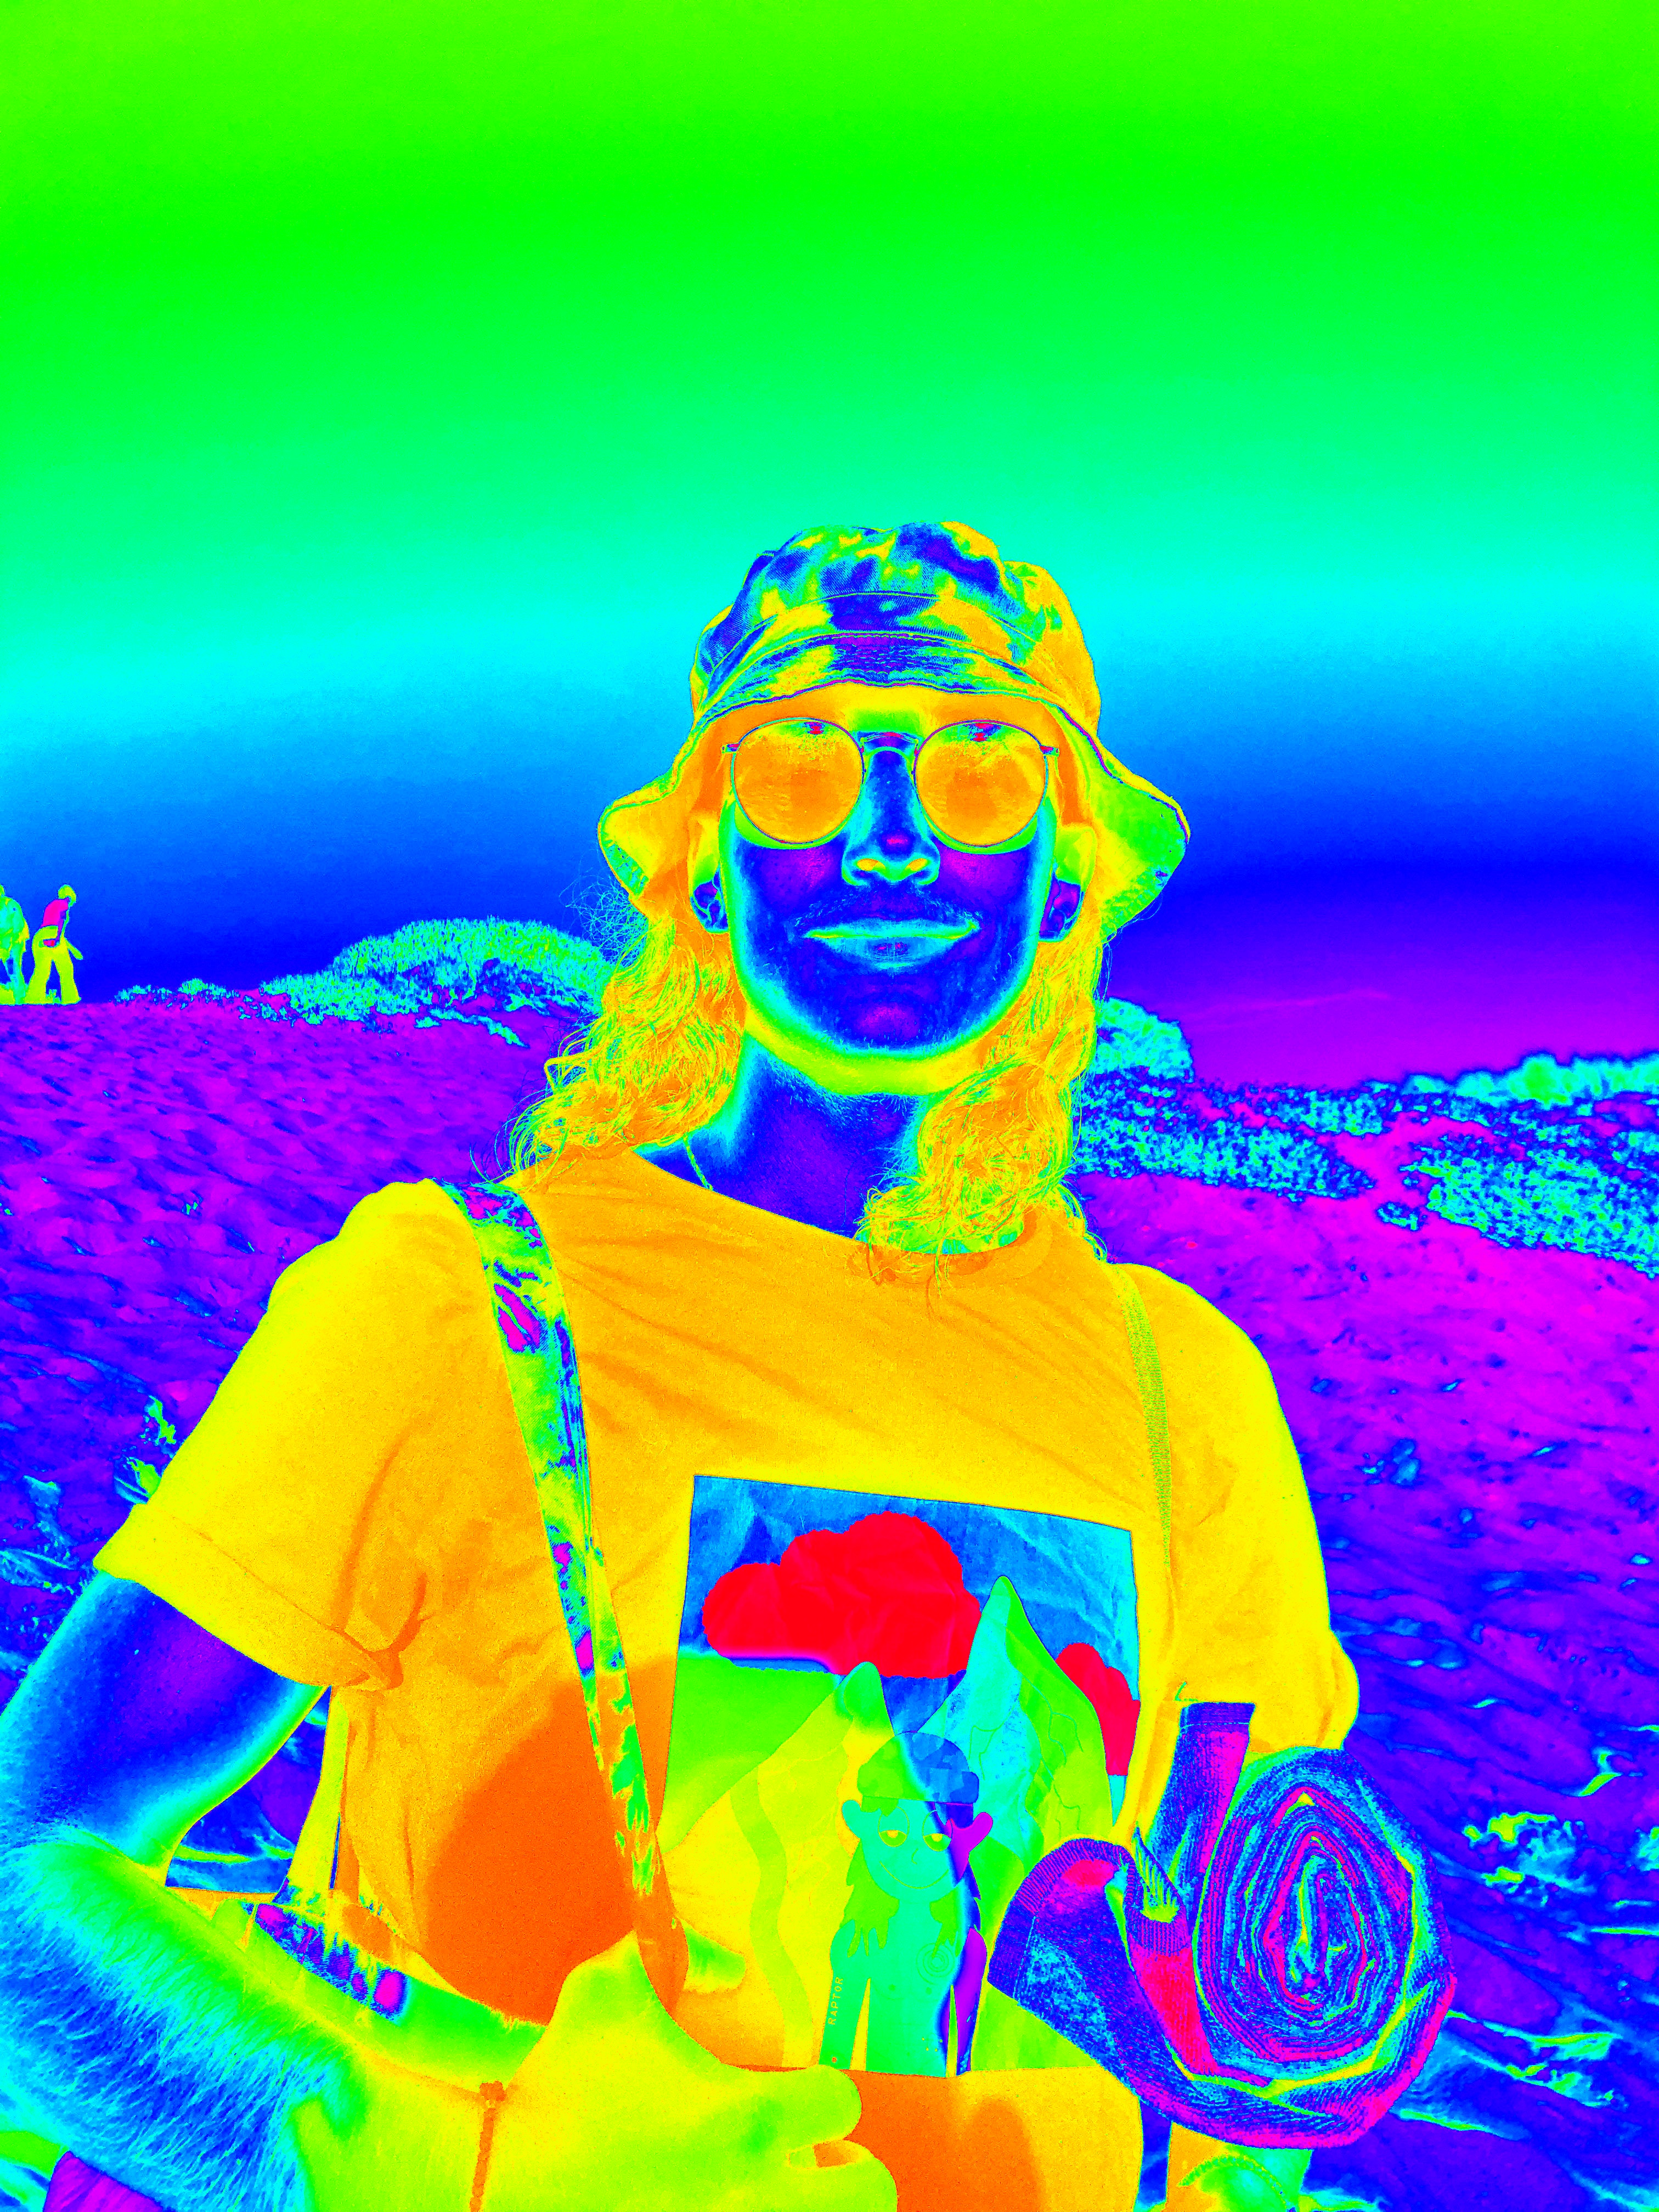
\includegraphics[width=.3\linewidth]{../Images/Output_Individual/Thermal1_Portrait.jpg}\label{Thermal1}}
	\subfloat[Thermal 2]{	\includegraphics[width=.3\linewidth]{../Images/Output_Individual/Thermal2_Portrait.jpg}\label{Thermal2}}\\
	\subfloat[Thermal 3]{	\includegraphics[width=.3\linewidth]{../Images/Output_Individual/Thermal3_Portrait.jpg}\label{Thermal3}}
	\subfloat[UV]{	\includegraphics[width=.3\linewidth]{../Images/Output_Individual/UV_Portrait.jpg}\label{UV}}
	
	\caption{ColourMaps Results}
	\centering
	\label{Images_ColourMaps}
	\end{figure}

	
	\subsection{Extra Effect \#2 - WaterColor}
	Method used: cv2.stylization(img, sigma\_s=100, sigma\_r=0.9)\\
	This effect can be seen in Figure \ref{WaterColor} and Figure \ref{ALLWaterColor}.
	\subsection{Extra Effect \#3 - Enhance}
	Method used: cv2.detailEnhance(img)\\
	This effect can be seen in Figure \ref{Enhance} and Figure \ref{ALLEnhance}.
	\subsection{Extra Effect \#4 - Glitch}
	This effect was implemented using a library called glitch\_this, by TotallyNotChase, found at \url{https://github.com/TotallyNotChase/glitch-this}. It is a command-line tool which reads in an image, and applies a glitch effect with a user-provided intensity, and optional scan lines too. I utilized the functionality in Jupyter that allows users to run terminal commands by using "!" before a line of code, and randomly generated the glitch intensity, and also whether or not the scan lines would be applied, in order to get varied results.\\
	This effect can be seen in Figure \ref{Glitch} and Figure \ref{ALLGlitch}.
	
	
	\begin{figure}[h]	
	\subfloat[WaterColor]{	\includegraphics[width=.3\linewidth]{../Images/Output_Individual/WaterColour_Portrait.jpg}\label{WaterColor}}
	\subfloat[Enhance]{	\includegraphics[width=.3\linewidth]{../Images/Output_Individual/Enhance_Portrait.jpg}\label{Enhance}}
	\subfloat[Glitch]{	\includegraphics[width=.3\linewidth]{../Images/Output_Individual/Glitch_Portrait.jpg}\label{Glitch}}	
		
	\caption{Extra Effects}
	\centering
	\label{Images_ExtraEffects}
	\end{figure}
		
%	\nocite{*}
%	
%	\bibliography{references}\addcontentsline{toc}{chapter}{References}
%	
	\chapter{References}
	\begin{enumerate}
		\item \url{https://programmerbackpack.com/python-opencv-building-instagram-like-image-filters/}
		\item \url{https://python.joho.info/image-processing/opencv-emboss-filter-py/}
		\item \url{https://ulwazi.wits.ac.za/courses/12061/assignments/72155?module_item_id=217456}
		\item \url{https://github.com/mbeyeler/opencv-python-blueprints/blob/master/chapter1/filters.py}
		\item \url{https://analyticsindiamag.com/converting-an-image-to-a-cartoon/}
		\item \url{https://www.tutorialspoint.com/cartooning-an-image-using-opencv-in-python}
		\item \url{https://www.askaswiss.com/2016/01/how-to-create-cartoon-effect-opencv-python.html}
		\item \url{https://data-flair.training/blogs/cartoonify-image-opencv-python/}
		\item \url{https://subscription.packtpub.com/book/application_development/9781785282690/1/ch01lvl1sec12/cartoonizing-an-image}
		\item \url{https://towardsdatascience.com/turn-photos-into-cartoons-using-python-bb1a9f578a7e}
		\item \url{https://www.geeksforgeeks.org/cartooning-an-image-using-opencv-python/}
		\item \url{https://towardsdatascience.com/using-opencv-to-catoonize-an-image-1211473941b6}
		\item \url{http://datahacker.rs/002-opencv-projects-how-to-cartoonize-an-image-with-opencv-in-python/}
		\item \url{https://medium.com/boundlessinfo/a-mini-project-with-opencv-in-python-cartoonify-an-image-d82b9ff6df70}
		\item \url{https://jrtechs.net/data-science/creating-pixel-art-with-open-cv}
		\item \url{https://www.programmersought.com/article/2697972427/}
		\item \url{https://subscription.packtpub.com/book/application_development/9781785283932/2/ch02lvl1sec23/embossing}
		\item \url{https://stackoverflow.com/questions/55508615/how-to-pixelate-image-using-opencv-in-python}
		\item \url{https://www.freecodecamp.org/news/sketchify-turn-any-image-into-a-pencil-sketch-with-10-lines-of-code-cf67fa4f68ce/}	
		\item \url{https://medium.com/analytics-vidhya/create-your-own-sketch-with-opencv-638a463c6ec6}
		\item \url{https://analyticsindiamag.com/converting-image-into-a-pencil-sketch-in-python/}
		\item \url{https://bastelhalde.de/post/creating-fake-thermal-images-using-python}
	\end{enumerate}
	
	\appendix
    \onecolumn
%APPENDIX A - MAIN
\chapter{Main Filters and Effects}
\label{MainEffectsAppendix}

\begin{enumerate}
	\item Cartoonify
	\item Pencil Sketch
	\item Pixelate
	\item Emboss
\end{enumerate}


\begin{figure}[h]
	\caption{Cartoonify}
	\centering
	\includegraphics[width=\linewidth]{../Images/Output_All/ALL_Cartoonify.jpg}
	\label{ALLCartoonify}
\end{figure}


\begin{figure}[h]
	\caption{Pencil Sketch}
	\centering
	\includegraphics[width=\linewidth]{../Images/Output_All/ALL_Pencil_Sketch.jpg}
	\label{ALLPencilSKetch}
\end{figure}


\begin{figure}[h]
	\caption{Pixelate}
	\centering
	\includegraphics[width=\linewidth]{../Images/Output_All/ALL_Pixelate.jpg}
	\label{ALLPixelate}
\end{figure}

\begin{figure}[h]
	\caption{Emboss}
	\centering
	\includegraphics[width=\linewidth]{../Images/Output_All/ALL_Emboss.jpg}
	\label{ALLEmboss}
\end{figure}





%APPENDIX B - EXTRA
\chapter{Extra Filters and Effects}
\label{ExtraEffectsAppendix}

\begin{itemize}
	\item ColorMaps
	\begin{itemize}
		\item Duo Chromatic
		\item Thermal 1
		\item Thermal 2
		\item Thermal 3
		\item UV
	\end{itemize}
	\item WaterColor
	\item Enhance
	\item Glitch
\end{itemize}

\begin{figure}[h]
	\caption{Duo Chromatic}
	\centering
	\includegraphics[width=\linewidth]{../Images/Output_All/ALL_Duo.jpg}
	\label{ALLDuo}
\end{figure}

\begin{figure}[h]
	\caption{Thermal1}
	\centering
	\includegraphics[width=\linewidth]{../Images/Output_All/ALL_Thermal1.jpg}
	\label{ALLThermal1}
\end{figure}

\begin{figure}[h]
	\caption{Thermal2}
	\centering
	\includegraphics[width=\linewidth]{../Images/Output_All/ALL_Thermal2.jpg}
	\label{ALLThermal2}
\end{figure}

\begin{figure}[h]
	\caption{Thermal3}
	\centering
	\includegraphics[width=\linewidth]{../Images/Output_All/ALL_Thermal3.jpg}
	\label{ALLThermal3}
\end{figure}

\begin{figure}[h]
	\caption{UV}
	\centering
	\includegraphics[width=\linewidth]{../Images/Output_All/ALL_UV.jpg}
	\label{ALLUV}
\end{figure}

\begin{figure}[h]
	\caption{WaterColor}
	\centering
	\includegraphics[width=\linewidth]{../Images/Output_All/ALL_WaterColour.jpg}
	\label{ALLWaterColor}
\end{figure}

\begin{figure}[h]
	\caption{Enhance}
	\centering
	\includegraphics[width=\linewidth]{../Images/Output_All/ALL_Enhance.jpg}
	\label{ALLEnhance}
\end{figure}

\begin{figure}[h]
	\caption{Glitch}
	\centering
	\includegraphics[width=\linewidth]{../Images/Output_All/ALL_Glitch.jpg}
	\label{ALLGlitch}
\end{figure}
	

\end{document}
